\documentclass[11pt]{article}

\usepackage[margin=1in]{geometry}
\usepackage{amsmath,amssymb,amsthm}
\usepackage{booktabs}
\usepackage{graphicx}
\usepackage{algorithm}
\usepackage{algpseudocode}
\usepackage{enumitem}
\usepackage{microtype}
\usepackage[numbers,sort&compress]{natbib}
\usepackage[colorlinks=true,linkcolor=blue,citecolor=blue,urlcolor=blue]{hyperref}

\newtheorem{proposition}{Proposition}
\newtheorem{assumption}{Assumption}
\newtheorem{definition}{Definition}

\newcommand{\uckv}{UCKV}
\newcommand{\calD}{\mathcal{D}}
\newcommand{\calS}{\mathcal{S}}
\newcommand{\calB}{\mathcal{B}}
\newcommand{\E}{\mathbb{E}}
\newcommand{\Prob}{\mathbb{P}}

\title{Uncertainty-Calibrated KV Cache Compression for Efficient LLM Inference}
\author{Draft manuscript}
\date{\today}

\begin{document}
\maketitle

\begin{abstract}
Key-value (KV) caching is essential for efficient autoregressive Transformer inference, but its memory footprint grows linearly with context length, batch size, number of layers, and number of attention heads. Existing KV cache compression methods typically decide what to retain from attention statistics, recency, layer structure, or quantization error. These signals are useful, but they do not explicitly account for when compression-induced changes are likely to be unsafe. This draft proposes \uckv{}, an uncertainty-calibrated framework for adaptive KV cache compression. \uckv{} treats cache compression as a selective memory decision: a calibrated risk model predicts whether a candidate cache budget will perturb the next-token distribution, and the system chooses the smallest budget below a risk tolerance, falling back to conservative retention when needed. We provide a formal problem statement, an attention perturbation bound linking discarded attention mass to output deviation, and a calibration-based risk-control argument. We also report controlled synthetic retrieval pilots using GPT-2 and SmolLM2-135M-Instruct. In the final SmolLM2 pilot, the selected tolerance $\epsilon=0.36$ matches the answer-containment accuracy of full-cache decoding and the strongest fixed sink-plus-window baseline on two held-out confirmation seeds, while reducing average retained tokens from 286.07 to 266.10 relative to full cache. These results are preliminary: they support uncertainty-calibrated budget selection as a promising operating point, but they do not yet establish wall-clock speedups or state-of-the-art long-context performance.
\end{abstract}

\section{Introduction}

Large language models (LLMs) are commonly served with autoregressive decoding. At each generation step, the model stores key and value activations from previous tokens so that later tokens can attend to them without recomputing the full prefix. This KV cache is one of the main practical reasons modern decoder-only Transformers can generate text efficiently. It is also a major memory bottleneck: cache size scales linearly with the number of processed tokens and with the number of concurrently served requests. As context windows and batch sizes grow, KV cache memory can dominate serving capacity, reduce throughput, and force systems to trade off latency, maximum context length, and the number of active users.

Recent work addresses this bottleneck through cache eviction, streaming attention, adaptive retention, and low-bit KV quantization. These methods exploit several empirical regularities: only a subset of tokens may receive most of the attention mass, initial tokens can act as attention sinks, recent tokens are often important, and key/value activations have compressible structure. However, compression is not merely an efficiency problem. A cache decision changes the information available to future attention layers. If the model is already uncertain, or if a query depends on evidence that is easy to evict, the same compression ratio may carry much higher reliability risk than it does for an easy continuation.

This project studies a simple question:

\begin{quote}
Can calibrated uncertainty estimates guide KV cache compression so that LLM inference becomes more efficient while preserving reliability under explicit risk controls?
\end{quote}

We propose \emph{Uncertainty-Calibrated KV Cache Compression} (\uckv{}). The central idea is to treat cache compression as a selective prediction problem over memory actions. At inference time, \uckv{} estimates a calibrated probability that an aggressive cache decision will harm the next generation step or the final task outcome. It then chooses a cache budget and token retention policy conditioned on this risk. High-risk steps receive larger budgets or fall back to conservative compression. Low-risk steps are compressed more aggressively.

This draft makes five initial contributions.

\begin{enumerate}[leftmargin=*]
    \item It formulates uncertainty-calibrated KV cache compression as a risk-constrained inference problem.
    \item It proposes a concrete \uckv{} method that combines calibrated uncertainty, adaptive budget allocation, sink/recent-token protection, and risk-weighted attention utility.
    \item It gives theoretical analysis connecting omitted attention mass to attention-output perturbation and connecting calibrated compression-risk estimates to expected degradation control.
    \item It implements a reproducible pilot pipeline for replay-based compression-risk estimation and free-running task evaluation.
    \item It reports controlled retrieval-only pilot results on GPT-2 and SmolLM2-135M-Instruct, including a final SmolLM2 tolerance sweep and two confirmation seeds. We explicitly mark which replay metrics are simulated and which task metrics come from real generated continuations.
\end{enumerate}

The current manuscript is therefore a research blueprint plus a first pilot report. Claims about empirical superiority are intentionally withheld: the current experiments are small and synthetic. They identify a reproducible operating point on controlled retrieval prompts, but larger long-context benchmarks and systems measurements remain future work.

\section{Related Work}

\paragraph{Transformer inference and KV-cache memory.}
The Transformer architecture replaces recurrence with self-attention and is the basis of modern decoder-only LLMs \citep{vaswani2017attention}. During autoregressive decoding, systems cache previous key and value activations so that each new token can attend to the prefix without recomputing all prior layers. This cache turns attention from repeated full-prefix computation into an incremental memory problem: latency and throughput depend not only on floating-point work, but also on how many KV blocks must be stored, moved, paged, and read at each step. FlashAttention reduces attention memory traffic through IO-aware exact kernels \citep{dao2022flashattention}, while PagedAttention and vLLM manage KV memory in blocks to improve serving throughput and reduce fragmentation \citep{kwon2023efficient}. Other serving systems address batching, offloading, speculative execution, and distributed scheduling, including Orca, FlexGen, and SpecInfer \citep{yu2022orca,sheng2023flexgen,miao2023specinfer}. \uckv{} is complementary to these systems: it asks which cache entries should be retained under a reliability constraint, rather than only how retained entries should be stored or scheduled.

\paragraph{Token eviction and adaptive KV-cache retention.}
Many KV-compression methods rely on the observation that not all prior tokens remain equally useful. Scissorhands exploits the persistence of token importance during generation \citep{liu2023scissorhands}. H2O retains heavy-hitter and recent tokens and frames eviction through a dynamic submodular perspective \citep{zhang2023h2o}. StreamingLLM protects attention sinks and recent tokens to support stable long streaming inference \citep{xiao2024streamingllm}. SnapKV selects prompt tokens from observation-window attention before generation \citep{li2024snapkv}; PyramidKV allocates layer-wise budgets using a pyramidal information-funneling observation \citep{cai2024pyramidkv}; Ada-KV studies adaptive head-wise budget allocation \citep{feng2024adakv}. Recent methods further explore semantic clustering, retrieval heads, expected future attention, and benchmark-driven tradeoffs \citep{devoto2025expected,yuan2024kvbenchmark}. These methods supply strong retention primitives, but most choose a compression level from efficiency or average-quality objectives. \uckv{} instead treats compression as a selective memory action: aggressive eviction is allowed only when calibrated risk estimates indicate that the current context and generation state can tolerate it.

\paragraph{KV-cache quantization, streaming, and hybrid compression.}
A second line compresses activations rather than removing tokens. KIVI studies asymmetric low-bit KV quantization and observes different structure in keys and values \citep{liu2024kivi}. KVQuant pushes ultra-low-bit cache quantization for very long contexts with outlier-aware handling \citep{hooper2024kvquant}. CacheGen compresses and streams KV cache state across serving boundaries \citep{liu2024cachegen}. Hybrid approaches combine eviction, mixed precision, streaming, or layer-wise allocation, making the design space increasingly rich. This matters for \uckv{} because uncertainty calibration need not be tied to a single compression primitive: the risk gate can choose among token retention budgets, quantization levels, or conservative fallbacks. In the present draft we focus on token retention because it is easier to instrument in replay experiments, but the formulation is intended to cover mixed eviction--quantization policies.

\paragraph{Reliability risks of cache compression.}
The motivation for risk-aware compression is strengthened by recent evidence that cache decisions can distort long-context evaluation itself. Long-context benchmarks reveal that models can underuse evidence in the middle of a prompt or fail as context length increases \citep{liu2024lost,bai2024longbench,hsieh2024ruler,zhang2024infinitebench,li2024needlebench}. A compression method can therefore appear efficient on easy prompts while silently amplifying failures on position-sensitive retrieval, multi-hop reasoning, or rare evidence. Dedicated KV-compression benchmarks and risk analyses make this point explicit: compression quality must be evaluated not only by memory reduction, but also by what accuracy, robustness, and calibration are lost in return \citep{yuan2024kvbenchmark,haverbeck2026risk}. This draft follows that stance. We report small pilot results as preliminary and avoid claiming superiority until larger long-context and task-diverse evaluations are completed.

\paragraph{Uncertainty estimation, calibration, and risk control.}
Calibration asks whether predicted confidence matches empirical correctness probability. Temperature scaling is a standard post-hoc baseline for neural classifiers \citep{guo2017calibration}, and selective prediction studies the risk--coverage tradeoff when a model abstains under high uncertainty \citep{geifman2017selective}. In LLMs, confidence can come from token probabilities, verbalized confidence, self-evaluation, multiple samples, semantic entropy, or external detectors \citep{kadavath2022language,farquhar2024detecting,manakul2023selfcheckgpt,geng2024survey}. Conformal risk control provides a distribution-free way to set thresholds for bounded downstream loss under calibration data \citep{angelopoulos2024conformal}. These ideas are usually applied to final answers or abstention decisions. \uckv{} moves the same principle inside inference: the system abstains from aggressive memory compression when the calibrated risk of harming generation exceeds a target tolerance.

\paragraph{Positioning of \uckv{}.}
The closest recent direction to this draft is confidence-aware KV management, including work that uses next-token uncertainty to adapt cache budgets \citep{li2026confkv}. Our project differs in emphasis. First, it frames budget selection as a calibrated risk-control problem rather than a heuristic confidence trigger. Second, it separates three measurable quantities: memory savings, task degradation, and calibration error of the compression-risk predictor. Third, it keeps a conservative fallback path, so negative results are informative: if uncertainty gates do not dominate H2O-like baselines under matched budgets, the paper should report the boundary conditions rather than hide them. This makes the current manuscript a reliability-centered study of KV compression, not only an efficiency method paper.

\section{Problem Formulation}

Consider a decoder-only Transformer with $L$ layers and $H$ attention heads per layer. For a sequence prefix $x_{1:t}$, each layer-head pair stores cached keys and values
\[
K_{1:t}^{\ell,h} = \{k_i^{\ell,h}\}_{i=1}^{t}, \qquad
V_{1:t}^{\ell,h} = \{v_i^{\ell,h}\}_{i=1}^{t}.
\]
At a decoding step $t+1$, a query $q_{t+1}^{\ell,h}$ attends over the cache with
\[
a_{t+1,i}^{\ell,h}
= \frac{\exp((q_{t+1}^{\ell,h})^\top k_i^{\ell,h}/\sqrt{d})}
{\sum_{j=1}^{t} \exp((q_{t+1}^{\ell,h})^\top k_j^{\ell,h}/\sqrt{d})},
\qquad
o_{t+1}^{\ell,h}
= \sum_{i=1}^{t} a_{t+1,i}^{\ell,h} v_i^{\ell,h}.
\]
A cache compression policy selects a retained index set $\calS_{t}^{\ell,h}\subseteq \{1,\ldots,t\}$, or a quantized representation of retained entries, subject to a memory budget $B_t^{\ell,h}$. In this first draft we focus on eviction-based compression; quantization is left as a planned extension.

Let $M(\pi)$ be the memory cost of a compression policy $\pi$, and let $D(y_{\mathrm{full}},y_{\pi})$ measure task or token-level degradation relative to full-cache decoding. Examples include answer mismatch, exact-match loss, negative log-likelihood increase, KL divergence between next-token distributions, or a human/LLM-judge factuality error indicator. Given a target degradation tolerance $\epsilon$ and an average memory budget $\bar{B}$, the ideal objective is
\[
\min_{\pi} \E[M(\pi)]
\quad \text{subject to} \quad
\Prob(D(y_{\mathrm{full}},y_{\pi}) > \delta) \le \epsilon,
\]
where $\delta$ defines an unacceptable compression-induced change.

This objective is difficult because full-cache outputs are not available at deployment, and task-level degradation may only be observed after generation. \uckv{} therefore learns a calibrated proxy:
\[
g_{\phi}(s_t,b) \approx \Prob(D_b > \delta \mid s_t),
\]
where $s_t$ includes uncertainty features, attention statistics, context length, layer/head summaries, and candidate budget $b$. At inference time, the policy chooses the smallest budget whose predicted risk is below a user-specified tolerance:
\[
b_t^\star = \min \{b \in \calB : g_{\phi}(s_t,b) \le \epsilon\}.
\]
If no candidate budget satisfies the tolerance, \uckv{} falls back to a conservative budget or full-cache decoding for that step.

\section{Method}

\subsection{Overview}

\uckv{} has two phases. In the calibration phase, a held-out set is decoded with full KV cache and with several candidate compression budgets. This produces supervision for both ordinary answer uncertainty and compression-induced degradation. In the deployment phase, \uckv{} uses the learned calibrators to allocate cache budgets and choose retained tokens.

\subsection{Uncertainty features}

For each decoding step $t$, let $p_t$ be the next-token distribution. A lightweight feature vector can include:
\[
\psi_t =
\left[
H(p_t),\,
1-\max_y p_t(y),\,
p_t^{(1)}-p_t^{(2)},\,
-\log p_t(y_t),\,
t,\,
\mathrm{len}(x)
\right],
\]
where $H(p_t)$ is predictive entropy, $p_t^{(1)}$ and $p_t^{(2)}$ are the top two token probabilities, and $-\log p_t(y_t)$ is available during teacher-forced calibration. For open-ended QA, a higher-cost optional feature is semantic uncertainty from multiple sampled answers \citep{farquhar2024detecting}. Since semantic uncertainty multiplies inference cost, the initial implementation should begin with token-level features and only add semantic features for analysis.

A calibrator $c_{\theta}$ maps $\psi_t$ to a calibrated error probability
\[
\hat{u}_t = c_{\theta}(\psi_t) \in [0,1].
\]
Possible calibrators include temperature scaling, isotonic regression, Platt scaling, or a small logistic model. Calibration quality should be reported with expected calibration error (ECE), Brier score, negative log-likelihood, and reliability diagrams.

\subsection{Compression-risk calibration}

Calibration data should include candidate cache budgets $b \in \calB$ and observed degradation labels:
\[
z_{t,b} = \mathbf{1}\{D_{t,b} > \delta\}.
\]
The compression-risk model estimates
\[
g_{\phi}(s_t,b) = \Prob(z_{t,b}=1 \mid s_t,b),
\]
where $s_t$ concatenates calibrated uncertainty $\hat{u}_t$, attention concentration statistics, omitted-mass estimates from candidate selection, context length, generation step, and budget. The risk model can be implemented as logistic regression for interpretability in the first version. If calibration is poor, the model should be post-calibrated with isotonic regression or conformalized on a split calibration set.

\subsection{Risk-aware budget allocation}

Let $\calB = \{B_1 < B_2 < \cdots < B_m\}$ be the allowed cache sizes. At step $t$, \uckv{} selects
\[
B_t^\star = \min \{B_j \in \calB : g_{\phi}(s_t,B_j) \le \epsilon\}.
\]
The tolerance $\epsilon$ controls a memory-reliability tradeoff. Smaller $\epsilon$ keeps more cache and should reduce compression risk. Larger $\epsilon$ allows more aggressive compression. A system-level scheduler can additionally enforce a global memory cap by adjusting $\epsilon$ or by using a dual variable that penalizes budget use.

\subsection{Token utility}

\uckv{} scores each cache entry with a combination of attention importance, uncertainty-weighted importance, recency, and protected positions. For token $i$ at step $t$:
\[
r_{i,t}^{\ell,h}
= \gamma r_{i,t-1}^{\ell,h}
+ a_{t,i}^{\ell,h} (1+\eta \hat{u}_t),
\]
where $\gamma \in [0,1]$ discounts old attention evidence and $\eta \ge 0$ increases the value of tokens attended to during uncertain steps. The final utility is
\[
U_{i,t}^{\ell,h}
= r_{i,t}^{\ell,h}
+ \lambda_{\mathrm{recent}}\mathbf{1}\{t-i < R\}
+ \lambda_{\mathrm{sink}}\mathbf{1}\{i \le S\}
+ \lambda_{\mathrm{ctx}}\hat{u}_{i}^{\mathrm{ctx}}.
\]
Here $R$ is a recent-token window, $S$ is the number of protected initial sink tokens, and $\hat{u}_{i}^{\mathrm{ctx}}$ is an optional calibrated uncertainty estimate from prefill. The retained set $\calS_t^{\ell,h}$ contains protected sink/recent tokens plus the highest-utility remaining tokens up to budget $B_t^\star$.

\subsection{Design variants}

The first experiments should compare three variants:

\begin{enumerate}[leftmargin=*]
    \item \textbf{\uckv{}-Budget}: uses uncertainty only to choose $B_t^\star$, while token scores follow an existing baseline such as H2O-style attention accumulation.
    \item \textbf{\uckv{}-Score}: uses a fixed budget but uncertainty-weighted token utility.
    \item \textbf{\uckv{}-Full}: combines risk-aware budget selection and uncertainty-weighted token utility.
\end{enumerate}

This separation is important because it tests whether gains come from adaptive memory size, better token selection, or both.

\section{Theoretical Analysis}

This section gives preliminary analysis. The goal is not to prove that uncertainty always identifies important cache entries, but to clarify what cache compression must control.

\begin{proposition}[Single-head attention perturbation]
Fix a layer-head pair and a decoding step. Suppose $\|v_i\|_2 \le V$ for all cached values. Let $a_i$ be the full-cache attention distribution and let $\calS$ be the retained set with retained attention mass $\alpha = \sum_{i\in\calS} a_i$. Let
\[
o = \sum_i a_i v_i,
\qquad
o_{\calS} = \sum_{i\in\calS} \frac{a_i}{\alpha} v_i,
\]
where $o_{\calS}$ is the attention output after renormalizing over retained tokens. If $\alpha>0$, then
\[
\|o-o_{\calS}\|_2 \le 2V(1-\alpha).
\]
\end{proposition}

\begin{proof}
We can write
\[
o-o_{\calS}
= \sum_{i\in\calS} a_i\left(1-\frac{1}{\alpha}\right)v_i
+ \sum_{i\notin\calS} a_i v_i .
\]
Taking norms and using $\|v_i\|_2\le V$ gives
\[
\|o-o_{\calS}\|_2
\le V\sum_{i\in\calS} a_i\left(\frac{1}{\alpha}-1\right)
+ V\sum_{i\notin\calS} a_i
= V(1-\alpha)+V(1-\alpha).
\]
\end{proof}

This bound supports attention-mass retention as a reasonable primitive: if a compression policy keeps the tokens carrying most of the full attention mass, the one-step attention output is stable. However, the bound is local. Errors can accumulate across heads, layers, and generation steps.

\begin{proposition}[Layer-wise accumulation sketch]
Assume each residual block after attention is $L_{\ell}$-Lipschitz with respect to its attention output, and assume the value norms in layer $\ell$ are bounded by $V_{\ell}$. If head $h$ in layer $\ell$ discards attention mass at most $\varepsilon_{\ell,h,t}$ at step $t$, then the hidden-state perturbation after $L$ layers is bounded by a constant multiple of
\[
\sum_{\ell=1}^{L}
\left(\prod_{j>\ell} L_j\right)
\sum_{h=1}^{H} 2V_{\ell}\varepsilon_{\ell,h,t}.
\]
\end{proposition}

The product term is loose but useful: cache errors in earlier layers may be amplified by later transformations. This motivates layer-wise and head-wise budget allocation rather than a uniform token budget.

\begin{proposition}[Risk selection under calibrated compression estimates]
Let $Z_b=\mathbf{1}\{D_b>\delta\}$ be the event that budget $b$ causes unacceptable degradation. Suppose $g_{\phi}(s,b)$ is calibrated up to error $\Delta$ on the deployment distribution in the sense that
\[
\left|\Prob(Z_b=1 \mid g_{\phi}(s,b)=q)-q\right| \le \Delta
\]
for all relevant $q$ and $b$. If the policy chooses any budget $b$ satisfying $g_{\phi}(s,b)\le \epsilon$, then
\[
\Prob(Z_b=1) \le \epsilon+\Delta.
\]
\end{proposition}

This proposition is an assumption-to-guarantee statement: the practical burden is to validate calibration and monitor distribution shift. It also suggests an abstention rule. If no budget has predicted risk below $\epsilon$, the system should use a conservative cache rather than silently compressing.

\section{Algorithm}

\begin{algorithm}[t]
\caption{Uncertainty-Calibrated KV Cache Compression (\uckv{})}
\label{alg:uckv}
\begin{algorithmic}[1]
\Require Model $f$, candidate budgets $\calB$, risk tolerance $\epsilon$, uncertainty calibrator $c_{\theta}$, compression-risk calibrator $g_{\phi}$, sink size $S$, recent window $R$, decay $\gamma$, uncertainty weight $\eta$
\State Initialize KV cache with the prompt prefill
\State Initialize token importance scores $r_{i,0}^{\ell,h}\gets 0$
\For{decoding step $t=1,2,\ldots$}
    \State Compute next-token logits and probability distribution $p_t$
    \State Compute uncertainty features $\psi_t$ and calibrated uncertainty $\hat{u}_t \gets c_{\theta}(\psi_t)$
    \For{each layer $\ell$ and head $h$}
        \State Estimate or observe attention weights $a_{t,i}^{\ell,h}$ over currently retained entries
        \State Update importance scores $r_{i,t}^{\ell,h}\gets \gamma r_{i,t-1}^{\ell,h}+a_{t,i}^{\ell,h}(1+\eta\hat{u}_t)$
        \For{each candidate budget $b\in\calB$}
            \State Build candidate retained set $\calS_{t,b}^{\ell,h}$ from sink tokens, recent tokens, and top utility scores
            \State Construct features $s_{t,b}^{\ell,h}$ including $\hat{u}_t$, attention concentration, context length, and budget $b$
            \State Estimate compression risk $\hat{r}_{t,b}^{\ell,h}\gets g_{\phi}(s_{t,b}^{\ell,h},b)$
        \EndFor
        \State Select $B_{t}^{\ell,h}\gets \min\{b\in\calB: \hat{r}_{t,b}^{\ell,h}\le \epsilon\}$
        \If{no candidate budget satisfies the tolerance}
            \State Set $B_t^{\ell,h}$ to the conservative maximum budget in $\calB$
        \EndIf
        \State Retain $\calS_t^{\ell,h}$ under budget $B_t^{\ell,h}$; evict non-retained entries from this layer-head cache
    \EndFor
    \State Sample or decode the next token and append its KV entries to the cache
\EndFor
\end{algorithmic}
\end{algorithm}

The algorithm is written at layer-head granularity. A lower-overhead implementation may share retained sets across heads, update importance scores every $k$ decoding steps, or perform prompt compression once after prefill and online compression only during generation. These engineering choices should be treated as ablations because they affect both quality and throughput.

\section{Experimental Design}

The full study should evaluate long-context quality, calibration, memory use, and throughput on standard benchmarks. This draft reports only a small synthetic retrieval pilot, described in Section~\ref{sec:pilot-results}. The broader protocol below is retained to make the intended study reproducible and to prevent accidental cherry-picking.

\subsection{Research questions}

\begin{enumerate}[leftmargin=*]
    \item \textbf{RQ1: Quality-efficiency tradeoff.} At the same memory budget, does \uckv{} preserve task quality better than non-calibrated cache compression baselines?
    \item \textbf{RQ2: Calibration.} Are the uncertainty and compression-risk estimates calibrated across datasets, context lengths, and answer types?
    \item \textbf{RQ3: Selective risk control.} Does lowering the risk tolerance $\epsilon$ monotonically reduce observed compression degradation while increasing memory use?
    \item \textbf{RQ4: Failure modes.} When \uckv{} fails, are errors associated with long-range retrieval, middle-position evidence, multi-hop reasoning, high entropy, or poor calibration?
\end{enumerate}

\subsection{Models}

Initial open-weight model candidates are Llama-2-7B/13B \citep{touvron2023llama}, Mistral-7B \citep{jiang2023mistral}, and Llama-3-8B if licensing and local hardware permit \citep{grattafiori2024llama}. The first implementation should start with one 7B-class model to stabilize instrumentation before scaling to additional model families.

\subsection{Datasets}

Long-context evaluation should use LongBench \citep{bai2024longbench}, RULER \citep{hsieh2024ruler}, and lost-in-the-middle style key-value retrieval placements \citep{liu2024lost}. Reliability-oriented evaluation should include TruthfulQA \citep{lin2022truthfulqa}, TriviaQA \citep{joshi2017triviaqa}, Natural Questions \citep{kwiatkowski2019natural}, and selected MMLU subsets \citep{hendrycks2021mmlu}. Language-modeling sanity checks can use WikiText-2 and C4-style held-out text if licensing and preprocessing are handled consistently.

\subsection{Baselines}

Baselines should include:

\begin{itemize}[leftmargin=*]
    \item full KV cache;
    \item sliding window and sink-plus-window retention;
    \item H2O-style heavy-hitter retention \citep{zhang2023h2o};
    \item Scissorhands-style persistent importance \citep{liu2023scissorhands};
    \item SnapKV-style prompt compression \citep{li2024snapkv};
    \item PyramidKV or Ada-KV style adaptive allocation where implementation is feasible \citep{cai2024pyramidkv,feng2024adakv};
    \item KIVI or KVQuant as optional quantization baselines or compositional extensions \citep{liu2024kivi,hooper2024kvquant}.
\end{itemize}

\subsection{Metrics}

Task quality metrics should follow benchmark conventions: exact match, F1, ROUGE, multiple-choice accuracy, retrieval accuracy, and perplexity where appropriate. Reliability metrics should include ECE, adaptive ECE, Brier score, negative log-likelihood, selective risk-coverage curves, and area under the risk-coverage curve. Efficiency metrics should include peak GPU memory, average KV cache bytes per request, tokens per second, time to first token, decode latency, and maximum batch size under a fixed memory limit.

\subsection{Pilot setup used in this draft}

The pilot uses controlled key-value retrieval prompts generated by the synthetic benchmark script in \texttt{experiments/}. Each prompt contains distractor text and one key-value pair, and the model is asked to return the value for a named key. Prompts vary across four context lengths (64, 128, 192, and 256 approximate words) and three answer positions (early, middle, and late). We use answer containment in the generated continuation as a simple task-level metric.

The final reported pilot uses SmolLM2-135M-Instruct with the tokenizer chat template, greedy decoding, and a 24-token generation budget. A main sweep uses 144 prompts from seed 29 and sink-plus-window candidates with four protected sink tokens and recent windows $\{32,64,128,\allowbreak 192,256,320,384\}$. The risk model is a logistic classifier trained on replay features to predict whether a candidate compression action causes step-level KL divergence above 0.01 relative to full-cache decoding. We tune \uckv{} risk tolerance on this main sweep and then run two confirmation seeds, 31 and 37, with 96 prompts each.

For each full replay run, the script logs full-cache greedy continuations, fixed-window replays, step-level KL divergence from the full-cache next-token distribution, top-1 mismatch, retained-token counts, logistic compression-risk calibration metrics, \uckv{} selections, and free-running compressed generations. Tolerance sweeps can reuse a fixed-window replay run and rerun only \uckv{} free-generation; those runs report real task generations but mark replay metrics as fixed-candidate simulations. The confirmation seeds report actual replay metrics for all policies.

\subsection{Reporting templates for full study}

The full-benchmark templates below remain placeholders. They define the intended reporting shape for future LongBench/RULER and reliability runs.

\begin{table}[h]
\centering
\caption{Quality-efficiency comparison template. Values are intentionally omitted in this draft.}
\begin{tabular}{lcccc}
\toprule
Method & KV budget & Task score & Peak memory & Decode tok/s \\
\midrule
Full KV & 100\% & TBD & TBD & TBD \\
Baseline compression & TBD & TBD & TBD & TBD \\
\uckv{}-Budget & TBD & TBD & TBD & TBD \\
\uckv{}-Score & TBD & TBD & TBD & TBD \\
\uckv{}-Full & TBD & TBD & TBD & TBD \\
\bottomrule
\end{tabular}
\end{table}

\begin{table}[h]
\centering
\caption{Calibration and selective-risk template. Values are intentionally omitted in this draft.}
\begin{tabular}{lcccc}
\toprule
Method & ECE & Brier & Risk at coverage & AU-RC \\
\midrule
Token entropy & TBD & TBD & TBD & TBD \\
Calibrated uncertainty & TBD & TBD & TBD & TBD \\
Compression-risk model & TBD & TBD & TBD & TBD \\
\bottomrule
\end{tabular}
\end{table}

\subsection{Ablations}

The ablation plan should vary uncertainty features, calibration method, risk tolerance $\epsilon$, sink size, recent window size, score decay $\gamma$, uncertainty weight $\eta$, per-head versus shared retained sets, and prompt-only versus online compression. For each ablation, report both quality and reliability metrics, not only memory savings.

\section{Pilot Results}
\label{sec:pilot-results}

This section reports controlled pilot results. They should be read as feasibility evidence for the proposed risk-calibrated selector, not as a claim of state-of-the-art KV cache compression. The experiments use small synthetic retrieval prompts and a small instruction-tuned model. Their role is to test whether the instrumentation works, whether risk tolerance behaves as a usable control knob, and whether a conservative \uckv{} operating point can match high-retention baselines while retaining fewer tokens.

\subsection{Metrics and evaluation protocol}

The pilot records two kinds of metrics. \emph{Replay metrics} force each compressed policy to follow the full-cache token path and measure the KL divergence and top-1 mismatch of next-token logits. These metrics isolate local distribution perturbation. \emph{Free-running metrics} let each compressed policy generate its own continuation and then check whether the expected answer string appears in that continuation. Free-running answer containment is closer to task behavior, but it remains a coarse metric on small prompt sets.

We use SmolLM2-135M-Instruct with the tokenizer chat template. Earlier raw-prompt runs gave poor full-cache retrieval accuracy and are treated only as diagnostics. This matters because cache compression comparisons are meaningful only after the full-cache prompt format is known to solve the task at a reasonable rate.

\subsection{Final SmolLM2 retrieval suite}

The final suite first runs a 144-prompt main sweep with seed 29. The fixed baselines are full cache and sink-plus-window retention with four protected sink tokens and recent windows $\{64,128,192,\allowbreak 256,320,384\}$. The \uckv{}-Budget sweep then reuses the fixed-window replay traces to evaluate risk tolerances from 0.30 to 0.50. The answer-containment metrics for the \uckv{} sweep are real free-running generations; the replay KL and top-1 mismatch metrics for those tolerance-sweep rows are fixed-candidate simulations from the source replay.

Table~\ref{tab:final-seed29} shows the main operating region. The best fixed-window baseline is sink+window 384, which matches full-cache answer containment at 0.9306 while retaining 283.93 tokens on average. \uckv{} at tolerance 0.36 also reaches 0.9306 answer containment, while retaining 259.21 tokens on average. Increasing the tolerance beyond 0.36 gives a sharp quality drop: tolerance 0.365 falls to 0.8889, and tolerance 0.40 falls to 0.7917. Thus the useful boundary is narrow but identifiable.

\begin{table}[t]
\centering
\small
\caption{Main SmolLM2-135M-Instruct retrieval sweep on seed 29, evaluation split. UCKV free-running answer containment is measured by real generation; UCKV replay metrics in this sweep are fixed-candidate simulations.}
\label{tab:final-seed29}
\begin{tabular}{lrrrr}
\toprule
Policy & Answer contain. & Avg kept & Avg KL & Fallback steps \\
\midrule
Full KV & 0.9306 & 287.60 & 0.0000 & 0 \\
Sink+window 256 & 0.7639 & 235.96 & 0.1300 & 0 \\
Sink+window 320 & 0.8472 & 267.14 & 0.0647 & 0 \\
Sink+window 384 & 0.9306 & 283.93 & 0.0006 & 0 \\
\uckv{} tol. 0.34 & 0.9306 & 274.13 & 0.0008 & 240 \\
\uckv{} tol. 0.35 & 0.9306 & 266.42 & 0.0009 & 181 \\
\uckv{} tol. 0.36 & 0.9306 & 259.21 & 0.0011 & 159 \\
\uckv{} tol. 0.365 & 0.8889 & 255.51 & 0.0013 & 153 \\
\uckv{} tol. 0.40 & 0.7917 & 237.65 & 0.0647 & 53 \\
\uckv{} tol. 0.50 & 0.6806 & 190.61 & 0.1389 & 20 \\
\bottomrule
\end{tabular}
\end{table}

\begin{figure}[t]
\centering
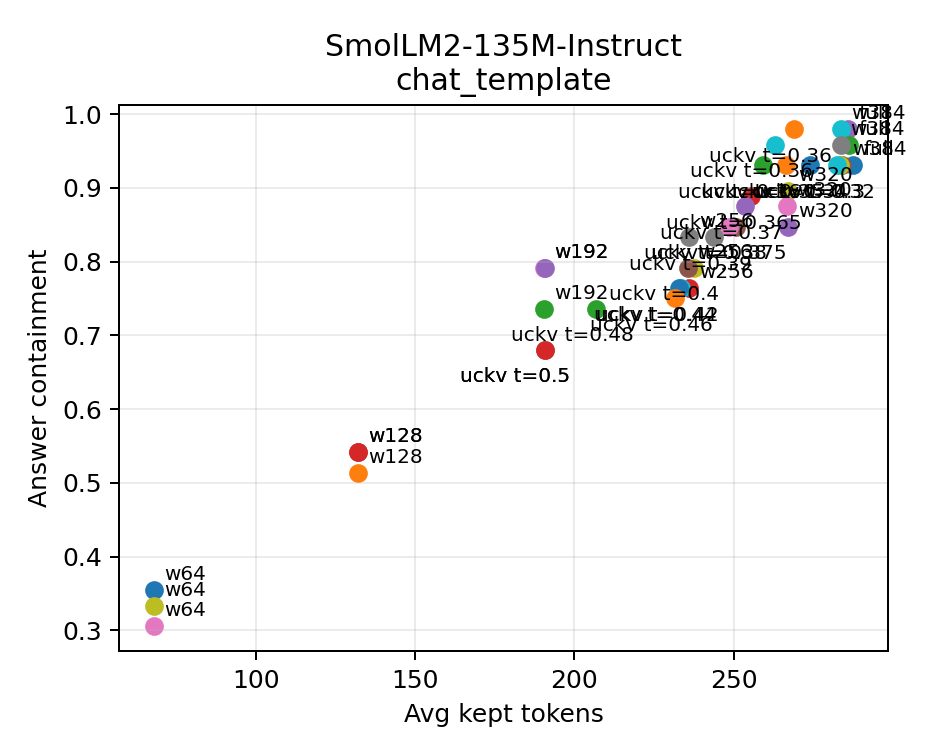
\includegraphics[width=\linewidth]{figures/retrieval-tradeoff.png}
\caption{Free-running retrieval tradeoff for the final SmolLM2 pilot. The selected operating point is \uckv{} tolerance 0.36: it matches the high-retention accuracy frontier on the main sweep while reducing retained tokens relative to full cache and sink+window 384.}
\label{fig:retrieval-tradeoff}
\end{figure}

\subsection{Confirmation seeds}

After selecting tolerance 0.36 from the seed-29 sweep, we run two confirmation seeds, 31 and 37, with 96 prompts each. These confirmation runs execute actual replay and actual free-running generations for all policies. Table~\ref{tab:final-confirm} reports the aggregate over the two confirmation seeds. \uckv{} matches the mean and minimum answer containment of both full-cache decoding and sink+window 384, while retaining fewer tokens on average.

\begin{table}[t]
\centering
\small
\caption{Confirmation seeds for SmolLM2-135M-Instruct, evaluation split. The selected \uckv{} tolerance is 0.36. Metrics are averaged across seed 31 and seed 37; all rows use actual replay and actual free-running generations.}
\label{tab:final-confirm}
\begin{tabular}{lrrrr}
\toprule
Policy & Seeds & Mean answer & Min answer & Avg kept \\
\midrule
Full KV & 2 & 0.9688 & 0.9583 & 286.07 \\
Sink+window 384 & 2 & 0.9688 & 0.9583 & 283.60 \\
\uckv{} tol. 0.36 & 2 & 0.9688 & 0.9583 & 266.10 \\
Sink+window 320 & 2 & 0.8854 & 0.8750 & 266.95 \\
Sink+window 256 & 2 & 0.8125 & 0.7917 & 235.79 \\
Sink+window 192 & 2 & 0.7917 & 0.7917 & 190.55 \\
Sink+window 128 & 2 & 0.5417 & 0.5417 & 132.00 \\
Sink+window 64 & 2 & 0.3438 & 0.3333 & 68.00 \\
\bottomrule
\end{tabular}
\end{table}

Relative to full cache, \uckv{} reduces retained tokens from 286.07 to 266.10, a 7.0\% reduction at the same answer-containment accuracy. Relative to the strongest fixed-window baseline, sink+window 384, it reduces retained tokens from 283.60 to 266.10, a 6.2\% reduction. These savings are modest, but they are achieved without reducing answer containment in the confirmation seeds.

\subsection{UCKV2 matched-budget gate}

The first \uckv{}-Budget pilots above identify useful instrumentation, but the resulting selector is conservative and does not directly compete with strong H2O-style heavy-hitter retention at a fixed cache budget. We therefore implemented a second-stage selector, denoted UCKV2 in the experiment code, that reuses the H2O attention-accumulation loop but gates attention updates by next-token uncertainty and adds prefill salience. This gate tests whether uncertainty can improve the heavy-hitter score itself, rather than only selecting among sink-window sizes.

The matched-budget gate compares H2O and UCKV2 at budgets $\{96,128,192,256\}$ on five independent SmolLM2 seeds, using 96 retrieval prompts per seed and the same chat-template, greedy decoding, and 24-token generation budget. Table~\ref{tab:uckv2-l1} reports evaluation-split answer containment averaged over seeds. The 256-budget point is the main signal: UCKV2 improves answer containment from 0.6708 to 0.8708 while retaining only 3.11 more tokens on average. The paired prompt comparison has 240 evaluation prompts; at budget 256, H2O is uniquely correct on 0 prompts and UCKV2 is uniquely correct on 48 prompts. A paired bootstrap gives a 95\% interval of $[0.1500,0.2542]$ for the answer-containment delta, and an exact McNemar test gives $p=7.11\times10^{-15}$.

\begin{table}[t]
\centering
\small
\caption{UCKV2 matched-budget gate on SmolLM2-135M-Instruct, evaluation split. Metrics are averaged over five seeds. ``Delta'' is UCKV2 minus H2O answer containment.}
\label{tab:uckv2-l1}
\begin{tabular}{rrrrrr}
\toprule
Budget & H2O answer & UCKV2 answer & Delta & H2O kept & UCKV2 kept \\
\midrule
96 & 0.4917 & 0.4667 & -0.0250 & 96.00 & 101.88 \\
128 & 0.4917 & 0.5167 & +0.0250 & 128.00 & 133.88 \\
192 & 0.5958 & 0.6042 & +0.0083 & 187.80 & 192.21 \\
256 & 0.6708 & 0.8708 & +0.2000 & 233.95 & 237.06 \\
\bottomrule
\end{tabular}
\end{table}

\begin{figure}[t]
\centering
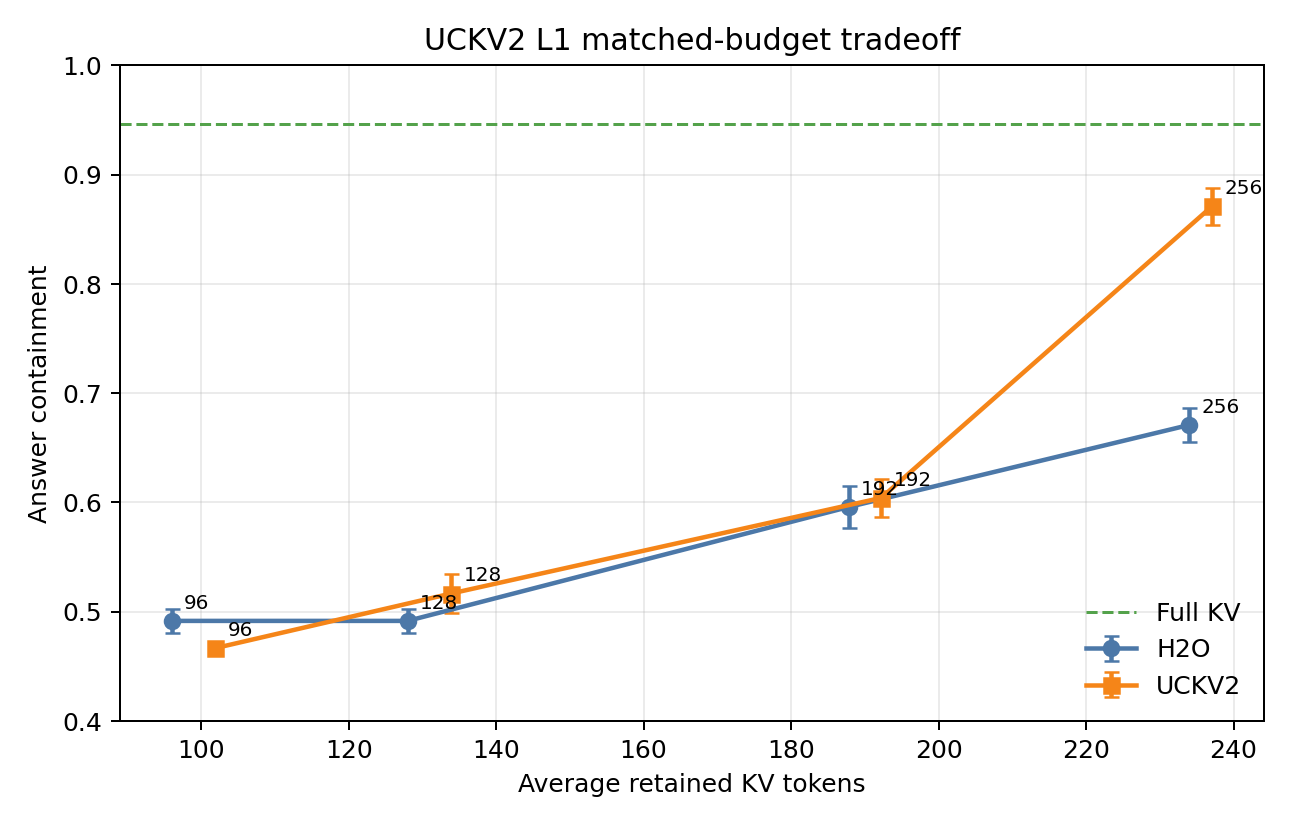
\includegraphics[width=0.86\linewidth]{figures/uckv2-l1-tradeoff.png}
\caption{UCKV2 matched-budget gate on SmolLM2-135M-Instruct. UCKV2 is not useful at the smallest budget, but it substantially improves the 256-token operating point relative to the H2O baseline.}
\label{fig:uckv2-l1-tradeoff}
\end{figure}

These local results are not a full benchmark claim. They are a gate for deciding whether the redesigned selector is worth a larger-model confirmation. The gate passes for budget 256, is weakly positive at 128 and 192, and fails at 96.

\subsection{Qwen2.5-7B confirmation of UCKV2}

We then ran the matched-budget confirmation on Qwen2.5-7B-Instruct on DGX Spark, using five independent seeds, 72 prompts per seed, the same controlled retrieval template, greedy decoding, and budgets $\{128,192,256\}$. This confirmation did not reproduce the SmolLM2 gain. Table~\ref{tab:uckv2-qwen25-7b} shows that H2O dominates the current UCKV2 selector at every tested budget: UCKV2 has lower answer containment, retains about 6.56 additional tokens, and incurs selector overhead during decoding.

\begin{table}[t]
\centering
\small
\caption{Qwen2.5-7B-Instruct DGX confirmation for UCKV2, evaluation split. Metrics are averaged over five seeds. ``Delta'' is UCKV2 minus H2O answer containment.}
\label{tab:uckv2-qwen25-7b}
\begin{tabular}{rrrrrr}
\toprule
Budget & H2O answer & UCKV2 answer & Delta & H2O kept & UCKV2 kept \\
\midrule
128 & 0.9444 & 0.6944 & -0.2500 & 128.00 & 134.56 \\
192 & 0.9333 & 0.7056 & -0.2278 & 192.00 & 198.56 \\
256 & 0.9278 & 0.7056 & -0.2222 & 256.00 & 262.56 \\
\bottomrule
\end{tabular}
\end{table}

\begin{figure}[t]
\centering
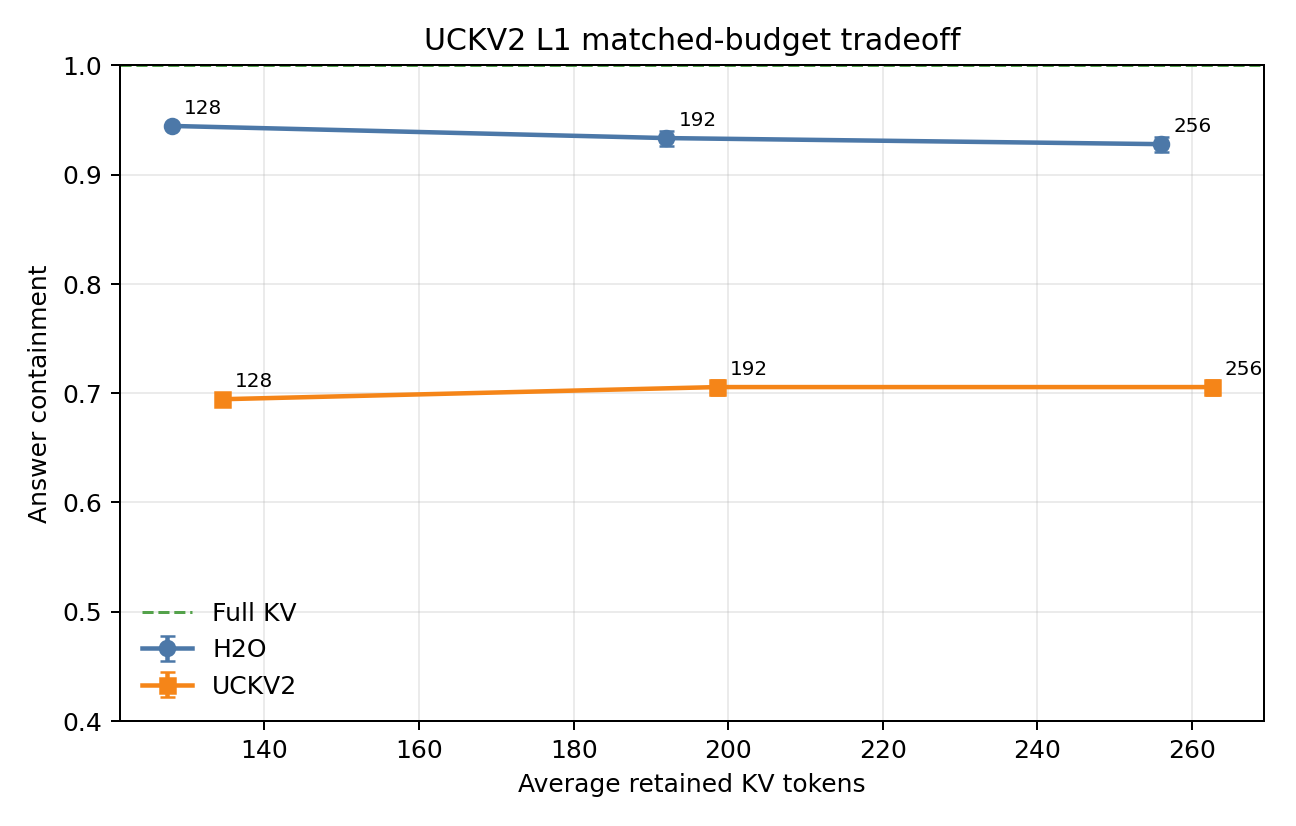
\includegraphics[width=0.86\linewidth]{figures/uckv2-qwen25-7b-tradeoff.png}
\caption{UCKV2 matched-budget confirmation on Qwen2.5-7B-Instruct. Unlike the SmolLM2 gate, the current UCKV2 selector is below H2O at all tested budgets on the 7B model.}
\label{fig:uckv2-qwen25-7b-tradeoff}
\end{figure}

The paired comparison contains 180 evaluation prompts. At budget 256, H2O is uniquely correct on 41 prompts, UCKV2 is uniquely correct on one prompt, the paired answer-containment delta is $-0.2222$, the bootstrap 95\% interval is $[-0.2833,-0.1611]$, and the exact McNemar test gives $p=1.96\times10^{-11}$. Thus the current UCKV2 selector fails the larger-model confirmation. We therefore treat the SmolLM2 result as a useful diagnostic signal, not as evidence that the current selector improves a 7B quality-memory frontier.

\subsection{Risk-tolerance boundary and failure modes}

The final sweep shows that tolerance is a real quality-efficiency control. From tolerance 0.34 to 0.36, answer containment remains at 0.9306 while average retained tokens fall from 274.13 to 259.21. At tolerance 0.365, answer containment drops to 0.8889, despite only a small additional token reduction. Larger tolerances continue to reduce retained tokens but degrade retrieval quality.

The position breakdown explains the cliff. At tolerance 0.36 on the seed-29 sweep, answer containment is 1.0000 for early-position answers, 0.8750 for middle answers, and 0.9167 for late answers. At tolerance 0.365, early-position containment falls to 0.8750 while middle and late positions remain unchanged. At tolerance 0.40, early-position containment falls to 0.5833. Thus the first visible failures come from evidence placement rather than from a uniform degradation across all prompts.

The context-length breakdown gives a complementary view. At tolerance 0.36, the seed-29 sweep retains high containment across context lengths: 0.8889 at 64 words, 0.9444 at 128 words, 1.0000 at 192 words, and 0.8889 at 256 words. For longer prompts, \uckv{} often falls back to the largest candidate window, which preserves quality but limits memory savings. This explains why the selected point is conservative.

\subsection{Pilot takeaways}

The pilot supports five modest conclusions. First, the replay/free-run pipeline can measure both local distribution perturbation and task-level degradation. Second, calibrated risk tolerance behaves as a usable memory-quality knob, with a clear boundary around 0.36 in the final SmolLM2 suite. Third, the selected \uckv{} point matches full cache and the strongest fixed-window baseline on the confirmation seeds while reducing retained tokens by 6--7\%. Fourth, uncertainty-gated heavy-hitter scoring can produce a strong local gain on SmolLM2, but the same selector fails on Qwen2.5-7B and is therefore not yet a validated scalable method. Fifth, the current implementation does not yet demonstrate broad benchmark or production serving speedups; the experiments measure retained-token counts, free-running answer containment, replay perturbation, and selector overhead on controlled runs.

The result is therefore useful but not yet positive enough for a main benchmark claim. It shows that uncertainty-calibrated cache control can be instrumented, stress-tested, and falsified under matched-budget conditions. The next method iteration should explain why the SmolLM2 gate does not transfer to Qwen2.5-7B, then retest only after a local matched-budget gate and a larger-model confirmation both pass.

\section{Discussion and Limitations}

\uckv{} depends on the quality of uncertainty estimates. Token entropy can be miscalibrated, especially after instruction tuning, temperature changes, domain shift, or decoding with sampling. Semantic uncertainty may be more aligned with answer-level risk, but it requires multiple generations and can erase some of the efficiency gains. A practical system may therefore need a two-tier design: cheap token-level uncertainty for every step and expensive semantic uncertainty only for high-risk prompts or offline calibration.

The pilot results highlight this limitation. SmolLM2-135M-Instruct required the tokenizer chat template before the full-cache baseline became meaningful. This is a reminder that compression experiments can be invalidated by prompt-format mismatch before cache policy is even considered. Future experiments should first verify that full-cache decoding solves the task at a reasonable rate, then compare compression policies.

Another limitation is observability. A compressed-cache model cannot know the attention mass it would have assigned to evicted tokens. The initial implementation should estimate this from pre-compression observations, periodic full-cache probes on calibration data, or attention statistics before eviction. This is a source of approximation error and should be measured.

The risk-control statement is only as strong as calibration under the deployment distribution. If prompts shift from short factual QA to long legal analysis, a previously calibrated risk model may become overconfident. Monitoring ECE and observed fallback rates over time is therefore part of the method, not an afterthought.

The current selector also has a practical limitation: the best pilot point is conservative. In the final SmolLM2 confirmation seeds, \uckv{} at tolerance 0.36 matches full cache and sink+window 384 on answer containment while reducing retained tokens by 6--7\%. This is useful as a risk-controlled baseline, but it is not yet a strong systems result. The selector still falls back frequently on longer contexts, and we have not measured wall-clock throughput or peak memory in a production-style serving stack. The next selector should explicitly trade off predicted risk and memory, rather than choosing the smallest candidate below a hard threshold.

Finally, \uckv{} should be evaluated against strong engineering baselines. A method that improves accuracy but adds enough overhead to reduce throughput may not be useful. The intended contribution is a better reliability-efficiency frontier, not compression at any cost.

\section{Follow-up Experimental Plan}

\begin{enumerate}[leftmargin=*]
    \item \textbf{Selector revision.} Replace the hard-threshold minimum-budget selector with a risk-memory objective, for example $\arg\min_b g_{\phi}(s_t,b)+\lambda M(b)$ or a fallback-penalized rule. The immediate target is to preserve the tolerance 0.36 task quality while reducing retained tokens and fallback frequency.
    \item \textbf{Position-aware diagnostics.} Add per-position calibration features or separate calibrators for early, middle, and late retrieval. The current pilot shows that early-position evidence is the first to fail when tolerance increases.
    \item \textbf{Calibration dataset.} Expand the held-out calibration split from the current controlled retrieval prompts to a larger mixture of synthetic retrieval, short QA, long-context QA, and summarization prompts. Continue reporting full-cache task quality before compression comparisons.
    \item \textbf{Deployable features.} Separate offline oracle features from deployable features. The current replay features are useful for pilot analysis, but a serving system should rely on features available during compressed generation.
    \item \textbf{Main benchmark run.} Compare full KV, sliding window, sink-plus-window, H2O-like retention, and \uckv{} variants on one 7B-class model across LongBench and RULER.
    \item \textbf{Reliability run.} Evaluate TruthfulQA, TriviaQA, Natural Questions, and MMLU subsets with calibration metrics and risk-coverage curves.
    \item \textbf{Scaling and systems run.} Repeat selected experiments on larger models or larger batch sizes, measuring peak memory, decode throughput, latency, and the overhead of risk prediction and cache slicing.
    \item \textbf{Paper revision.} Add statistical uncertainty, include failure-case examples, and revise claims to match observed evidence.
\end{enumerate}


\bibliographystyle{plainnat}
\bibliography{references}

\end{document}
